\documentclass[11pt]{article}
% \usepackage[top=1in,bottom=1in,left=1in,right=1in]{geometry}
\usepackage[margin=1in,paperwidth=8.5in,paperheight=11in]{geometry}
\usepackage{amsfonts}
% Macros are user defined texts or eqn's that are repeated, Modularity implemented
% Macros shouldnt have the first letter to be the same
\def\cs_eq{y=\Phi*x}
\def\exp{Holy Grail of CS:}
% Graphics Package
\usepackage{graphicx}

\begin{document}
\tableofcontents
%  Specify table of contents above all the declarations
%   /* use \_ space after '\' usage so that, the particular character is evaluated */
\title{\LaTeX \ 101}
\author{Sathyaprakash Narayanan}
\date{\today}
\maketitle

Hello World !! \\
To use mathematical symbols $\mathbb{N,R,S,Z}$ \\
This is my first Latex document. \\
Using Macros like, \exp \ $\cs_eq$

\section{Math Function}
My math functions as $(y=\Phi*x)$ and $e=mc^2$ \\

My math functions as $$(y=\Phi*x)$$ and $$e=mc^2$$


superscript : $$2x^{3x+4}$$ /*inline math function*/

subscripts :  $$ \Sigma^{i=1,j=14}_{i=m,j=n}*x_{i,j} = \int 4(x^{i,j}) $$

\begin{center}
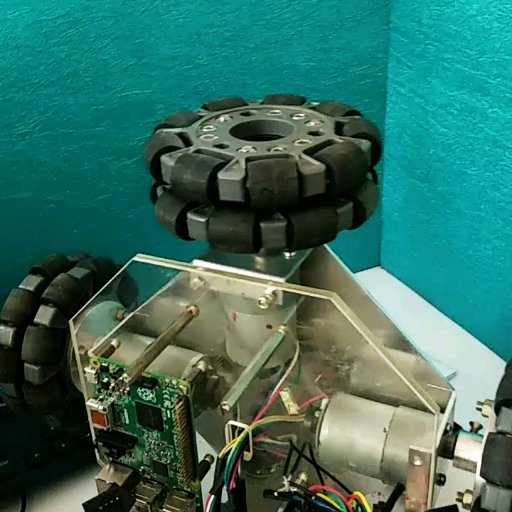
\includegraphics[width=5in,height=5in]{robo.jpg}
\end{center}
%  roatate with ``angle=...''
\begin{center}
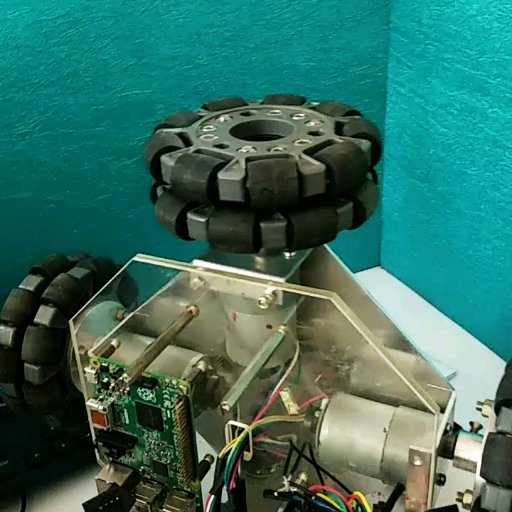
\includegraphics[scale=0.5,angle=45]{robo.jpg}
\end{center}
greek letters :

$$\alpha,\beta$$
$$ y= \sqrt[5]{\sin{x}*\log_4{x}} $$

$$ h(v)=\frac{1}{\sqrt{1+\sqrt{x}}} $$

$ y= \displaystyle{\frac{4}{3}}$     %/* display style increases the font size of the math*/
$$ \frac{1}{x^2+\sqrt{\frac{x}{2}}+1}$$


\section{Fractions}

$$ (2+x) * \left\{\frac{x}{u}\right\} =\$12.478$$ 
dollars \\
$$ \left|\frac{x}{|x|+1}\right|$$

$$\left. \frac{dy}{dx}\right|_x=0$$

\section{Tabulation}
\begin{tabular}{|c|c|c|c|c|c|c|}
\hline 
$x$ & 1 & 2 & 3 & 4 & 5 & 6 \\ \hline
$f(x)$ & 10 & 11 & 12 & 13 & 14 & 15  \\ \hline
\end{tabular}

\section{Equation Array}
\begin{eqnarray}
4x^2+5=5 \\
x^2=(-2) \\
x=2i \\
\end{eqnarray}
% /* align all equations */
\begin{eqnarray}
 4x^2+5&=&5 \\
x^2&=&(-2)\\ 
x&=&2i
\end{eqnarray}
% /* without the legendary numbers*/
\begin{eqnarray*}
 4x^2+5&=&5 \\
x^2&=&(-2)\\ 
x&=&2i
\end{eqnarray*}

\section{Lists}
\begin{enumerate}
 \item pencil
 \item pod
    \begin{itemize}
     \item space
     \item ground
        \begin{itemize}
         \item pop
         \item jor
         \item gor
        \end{itemize}
    \end{itemize}
 \item paper
\end{enumerate}
 
 
 \begin{enumerate}
  \item [hey :]$(a+b)=(b+a)$
  \item[commutative :] $(a+(b+c))=((a+b)+c)$
 \end{enumerate}

\section{Text Format}
This will produce \textit{italicized} text. \\
This will produce \textbf{bold-faced} text. \\ 
This will produce \textsc{small caps} text. \\
Please visit \texttt{typewriter} text.    \\
To add url's use \texttt{http://satabiossathya.weebly.com} \\
To increase the size of the font \begin{large}Larger \end{large} \\
To increase the size of the font even \begin{Large} Larger \end{Large}     \\
To increase the size of the font even even\begin{huge} Larger \end{huge}  \\

/* small -- > tiny are the right opposites of the above operations. */

\begin{center} 
center the statement we use.  \\
\end{center}

\begin{flushleft}
 To left centrize the statement. \\
\end{flushleft}

\begin{flushright}
 To right indent the statement. \\
\end{flushright}



\section{Sections}
  \section{First}
   \subsection{Linear Function}
     \subsection{Standard Form}
      \subsection{Vertex Form}





\end{document}
